\section{Wednesday, July 10, 2019}

\subsection{Process Control Terminology}

Before we get started with process control, we need to introduce some new terminology.

The \vocab{kernel} is a component of the operating system that's responsible for maintaining security, performing file management, and managing processes. It's like the ``manager'' of the operating system---it enforces ``policies.''


When a program is running, there are various tasks that we don't consider to be sensitive (i.e. dangerous to the operating system). Hence, the program doesn't require too many permissions. We say that these programs are run in \vocab{user mode}. When we're executing a program in user mode, we can't perform any sensitive (dangerous) operations, and we don't have the privilege of accessing everything associated with the operating system. 


By contrast, some instructions are restricted so that only the operating system itself can execute them. When a program has this privilege, we say that the program is running in \vocab{kernel mode}. Some examples of operations a program can perform that requires kernel mode include halting the CPU or performing I/O.


\vocab{Context switching} is a feature utilized by an operating system to store the state of a process so that it can be restored and its execution can be resumed from the same point at a later time. This happens really fast, so it seems almost as if we're performing multiple tasks at the same time. For example, if we've got a single CPU, and we're programming while listening to music, our CPU would be rapidly context switching the two processes. What dictates how the context switch chooses which processes to pause and resume? The kernel does.

\subsection{System Calls}

A \vocab{system call} is a special function that allows us to interact with the kernel. Functions that permit us to perform file I/O, create processes, and read the system clock all perform system calls.

System calls aren't the only way in which we can interact with the kernel. We can also use the shell, which allows for indirect interaction (when we're copying or moving files, we're interacting with the kernel). Are there different types of shells? Yes - so far, we've been using the \vocab{tcsh shell}; however, \vocab{bash} and \vocab{korn} are also shells (to change to either of these shells, we can execute the \verb!bash! or \verb!ksh! commands in Unix).


\subsection{Processes vs. Threads}

A \vocab{thread} is an execution path, almost like a program inside of another program. For example, suppose we've designed a clock that works in our own timezone. But now, we want to design four clocks, each of which represent a different timezone. We've already got one working clock, so we can spawn four threads, each of which represent a different timezone. The program will allow each thread to run for the correct amount of time.


Here's another example. Suppose we're computing the sum of an array. We can use one thread to compute the sum of the first half, and a second thread to compute the sum of the second half. Depending on our hardware, this can save time. 



What's the difference between a thread and a process? Threads lives inside of a process. The most minimalistic representation of a thread includes the stack (used to support function calls) and the program counter. We can have multiple threads helping us run a process with context switching. 

Something key thing to note is that threads share the same resources. That is, if a process opens a file, all of the threads share the same file. Moreover, if a process dynamically allocates memory, all of the threads have access to the memory (the heap and global variables are shared by all of the threads). 

A real life analogy is a household. A house can be viewed as a process, whereas the people inside of them are the threads. Everything inside of the house (process) is shared by the people (threads). 


Every process goes through several states during its execution. Collectively, these states are referred to as the \vocab{process life cycle}. A pictorial representation of this life cycle is presented below:

\begin{center}
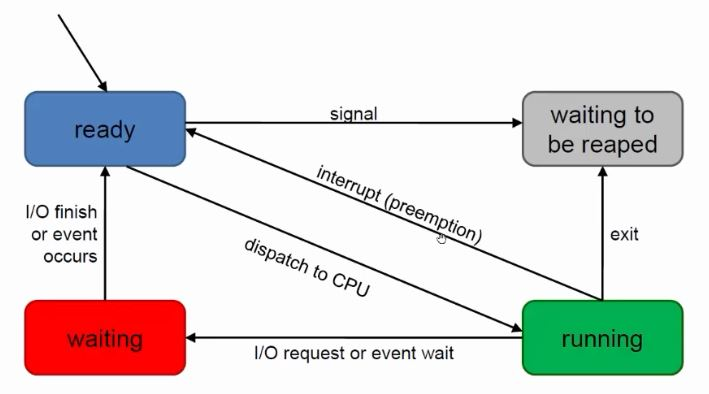
\includegraphics[width=\textwidth]{july10/pls}
\end{center}

What's happening here? \begin{itemize}
    \item When a process is in the \vocab{ready state}, it is not currently executing; however, it is ready to begin executing. It is waiting for the kernel to tell it to start running.
    \item Once the kernel tells the program to run, the process moves to the \vocab{running state}. What can happen from here? The program might move into the \vocab{waiting state}, where it awaits I/O. Alternatively, the program can finish executing and move to the \vocab{waiting to be reaped} stage. Finally, there's one last scenario: the program can be interrupted (by perhaps the programmer). If this happens, the process moves from the running stage back to the ready stage.
    \item Let's say our program takes in user input. Once it starts running, it'll move to the waiting state. Interestingly, once the I/O is completed, the program can't immediately go back to the running state again. It needs to go back in line to the ready state before it can go back into the running stage. 
\end{itemize}



\subsection{Signals}

A \vocab{signal} is a method that allows two processes to communicate. A process is able to recognize when it receives a signal, and the process is able to react in response to that signal. 

We've already been using signals: \verb!CTRL + C! is a signal, and the program responds by terminating. Formally, the name of this signal is \verb!SIGINT!. 

Some other signals that are used by the kernel include the following: \begin{itemize}
    \item \verb!SIGSEGV! is a signal indicating a segmentation violation (a.k.a. segmentation fault)
    \item \verb!SIGFPE! is a signal used to indicate a floating point exception.
    \item \verb!SIGCHILD! is a signal used to indicate that a child process has terminated.
\end{itemize}

A program doesn't necessarily terminate when it receives a signal --- it completely depends on the signal being sent.

\subsection{Creating Processes}

In Unix, a new process (called a \vocab{child}) is created by an existing process (called a \vocab{parent}), making a parent-child relationship between the two processes. The new child process will then be able to execute the program we want. 

How do we create a new process? The system call do create a new process is \verb!fork()!. This call creates a copy of the parent process. 

What gets copied when we fork a process? Just about everything: \begin{itemize}
    \item All variables (the entire address space) gets copied.
    \item The point of execution is copied (i.e. parent and child processes continue execution after the fork system call)
    \item The file descriptor table (files opened by the process) is copied.
\end{itemize}

The stack, heap, data, and code all get executed.



What are the benefits of forking if we're getting the same exact thing? Well, once we've forked a program, we can modify the child process and change it to a different program. This is done wit a system call that we'll see later on.

Let's look at an example in C:

\lstset{
caption=Forking 1
}
\begin{center}
\lstinputlisting[language=c]{july10/july1001.c}\label{Forking Example 1}
\end{center}

First off, the \verb!pid_t! data type represents a signed integer used for process identification. (The \verb!_t! portion of a data type means that the data type is internally mapped to an integer). Thus, we can print the variable \verb!result! using the \verb!%d! format specifier. 

Next, we set \verb!result! to \verb!fork()!, which returns a signed integer. The \verb!fork()! function returns a duplicate process of the program currently being executed. Once this \verb!fork()! takes place, the processes will exist, and they will be executing after the function call. It doesn't concern us which process is executing first. All that we know is that we'll have two processes, both of which will be executing after Line $12$. 

Now, what's the return value of \verb!fork()!? It's the Process ID (PID) associated with the child process. If we again were to call \verb!fork()! on a child, the return value would be zero: the PID of a child process is always zero. So, the variable \verb!result! has two different values: the PID of the child process in the parent process, and $0$ in the child process.

Can forking fail? Yes. There is a limit to the number of processes we can fork since space is limited. If the fork fails, $-1$ is returned, which is why we have the conditional from Lines $13$ to $15$.

Finally, the program prints the PID of the newly created child process. 


Here's another example:

\lstset{
caption=Forking 2
}
\begin{center}
\lstinputlisting[language=c]{july10/july1002.c}\label{Forking Example 2}
\end{center}

This time, before we fork our process, we declare the variables \verb!x! and \verb!p!. We also dynamically allocate memory for \verb!p!. Now since forking copies all components of the code, our new process will also have these variables. The only difference is that the variable \verb!result! will be the PID of the child process for the parent process, and it will be $0$ for the child process. We can use this fact to produce different outputs.

By comparing the PID to $0$, we can obtain different outputs between the child and parent processes (for the child process, the Boolean expression \verb!result == 0! will evaluate to true). In the program above, we'll increase the variable \verb!x! to $21$ for the child process; the variable \verb!x! will remain $20$ in the parent process. 


Since we've dynamically allocated memory prior to forking, our child process has inherited this new memory area as well. So, we need to call \verb!free()! in both the child and parent process (somewhere that's accessible by both processes). 

One thing that is strange, however, is that when we print the address of the pointers, we'll obtain the same memory address. It'll appear as if the pointer \verb!p! is pointing to the same place for both the child and parent process. However, this is not the case --- the operating system will convert them to distinct areas in memory when it is needed.


Something else to note is that even though the \verb!fork()! came after the variable declarations, the child process still inherits all of the variables that come before it. The only thing determined by \textit{where} the \verb!fork()! call comes is where the point of execution for the child process is set to.


The \verb!getpid()! and \verb!getppid()! functions return the PID of the process currently executing that function. What happens if we call \verb!getppid()! on a process that doesn't have a parent? The PID of the the shell will be returned---the shell is the ancestor of all processes.


Recall that the newline character, \verb!\n!, is used to flush the buffer. If we use \verb!printf! without the new line character, whatever we're printing is placed in memory; it isn't printed until the buffer is flushed. So, if we print a statement without flushing the buffer prior to forking a process, the buffer also gets duplicated. Consequently, if we perform another \verb!printf! statement (after the \verb!fork! call), the message that came before the \verb!printf! will be printed twice. Long story short, it's usually a good idea to make sure the buffer has been cleared prior to forking. 


Now let's look at an application of forking:

